\documentclass{article}
\usepackage[T1]{fontenc}
\usepackage{lmodern}
\usepackage{graphicx}
\usepackage{amsmath,amssymb}
\usepackage[a4paper,margin=2cm]{geometry}
\usepackage[absolute,overlay]{textpos}
\setlength{\TPHorizModule}{1mm}
\setlength{\TPVertModule}{1mm}
\usepackage[indonesian]{babel}
\usepackage{hyperref}
\setlength{\emergencystretch}{2em}
% unit: Halaman 38

\begin{document}

% === Halaman 38 (python/native) ===

38

Mode CFB

Enkripsi:

Cj = Pj MSBs(EK (Xj))

Xj+1 = LSBb – s(Xj) || Ci

Dekripsi:

Pj = Ci MSBs(EK (Xj))

Xj+1 = LSBb – s(Xj) || Ci

Mode CFB mengoperasikan block cipher seperti stream cipher!!

% deskripsi: gambar native xref 165
\noindent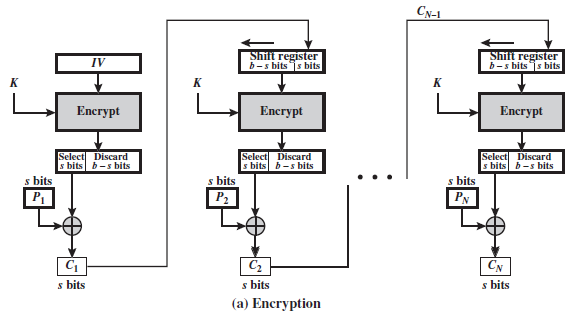
\includegraphics[width=0.85\textwidth]{../../images/python/page_038_img_01.png}

% deskripsi: gambar native xref 166
\noindent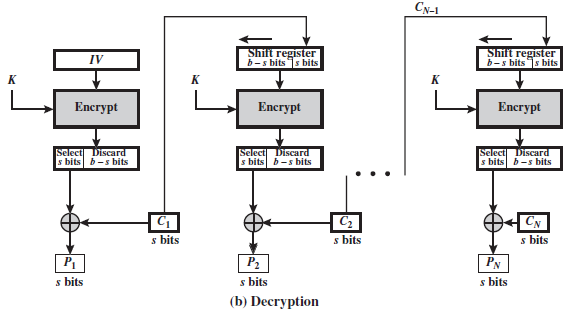
\includegraphics[width=0.85\textwidth]{../../images/python/page_038_img_02.png}

\end{document}
